\section{Задачи и алгоритм коллективной экспертизы}

\begin{frame}{Задача коллективной экспертизы: варианты}
 \vspace*{-3mm}
	\begin{enumerate}
		\item 
		Методы поиска оценки, близкой в среднем квадратичном к оценкам различных экспертов\footnote{Пытьев\;Ю.\,П. \emph{Эмпирическое восстановление мер возможности и правдоподобия возможности в моделях экспертных решений}, 2009}:
% .}~// Докл. АН СССР, Т.\;224, \No 6, С.\;1283--1286, 2009.\\}: 
		метод матриц попарных сравнений, векторов перестановок  и др.;
	%	\item Новый метод -- метод векторов предпочтений; %новый для т.\,в.~Пытьева
		\item
		Аналогичный метод -- метод векторов предпочтений;
		\item
		Новый метод -- введение отношения квазипорядка (частичного порядка с точностью до эквивалентности) на множестве распределений нечёткого элемента и вычислние верхней грани распределений.
	\end{enumerate} 
	
	 \vspace*{-2mm}
	{ \small Коллективное мнение экспертов с помощью матриц попарного сравнения: 
	\\ $\big(  \p^{(r)}(\cdot)$ -- совместное распределение на основе оценок эксперта $r = 1 \ldots R \big)$ 
	 \vspace*{-2mm}
	\begin{columns}
	   \column{0.5\textwidth}
	      \begin{gather*}
		   m^{(r)}_{kj} = \begin{cases}
			\;\;\;1,\;\; \p^{(r)}(t_k) > \p^{(r)}(t_j)\\
			\;\;\;0,\;\; \p^{(r)}(t_k) = \p^{(r)}(t_j)\\
			-1, \;\; \p^{(r)}(t_k) < \p^{(r)}(t_j)
		  \end{cases} 
		  \\ k,j = 1\ldots\abs{T}+1; 
		  \\ \text{причём }\p^{(r)}(t_{\abs{T}+1}) \define= 0.  
	      \end{gather*}
	   \column{0.5\textwidth}
	     \vspace*{-3mm}
	      \begin{gather*}
		  m_* = \arg \min_m \sum_{r=1}^{R} \rho(m^{(r)}, m),
		  \\ \text{где } \rho(m, m') = \left( \sum_{k,j=1}^{\abs{T}+1}(m_{kj} - {m'}_{kj})^2 \right)^{1/2}.
		  \\ \text{$m_*$ не всегда просто найти!}
	      \end{gather*}
	\end{columns}  } 
\end{frame} %===========================



   % \begin{tikzpicture}
  %    \begin{axis}[
%	width = 0.5\textwidth, height = 0.4\textwidth,
 %   xlabel = {$L$},
%    ylabel = {$\alpha$},
	%ymin = 0, ymax = 0.4,  % if left default there will be margins
	%xmin = 2, xmax = 30,
 %   xtick = {2, 6, 10, 14, 18, 22, 26, 30}
%	xticklabels = {,,},
%	yticklabels = {,,}
%	]
%	\addplot[blue, very thick] table[x=n, y=cone] {./pic/results.txt};
%	\addplot[dash pattern=on 6pt off 3pt on 1pt off 3pt] table[x=n, y=svm] {./pic/results.txt};
%     \end{axis}
 %   \end{tikzpicture}


\begin{frame}{Квазипорядок распределений возможностей}
	\begin{columns}
	  \column{0.6\textwidth}
	    \begin{gather*}
	    \p^{(1)} \prec \p^{(2)} \text{ (читается <<уточняет>>) } \Leftrightarrow \\ 
	     \Leftrightarrow
	    \begin{cases}
 		  \supp\;\p^{(2)} \supset \supp \; \p^{(1)};
		  \\[0.8ex]  \exists \gamma: \p^{(2)}(t) = \gamma(\p^{(1)}(t)),\;  \mathsmaller{ t\, \in\, \supp\;\p^{(1)}}; 
		 \\[0.ex] \mathsmaller{\gamma: \zo \rightarrow \zo \text{ -- монотонная непрерывная,} } 
		%  \\ \hspace{10ex}
		   \mathsmaller{\gamma(0)=0,\; \gamma(1)=1};
		 \\[0.8ex]  \p^{(2)}(t') \leq \p^{(2)}(t),\;  \mathsmaller{t'\, \in\, T\, \setminus\, \supp \; \p^{(1)},\;  t\, \in\,  \supp \; \p^{(1)}}.
	    \end{cases}
	    \end{gather*}

	    \begin{center}
	      \vspace{2mm}
		При достаточно общих условиях %множества решений {\em задачи выбора} вложены:
		\\[0.5ex] 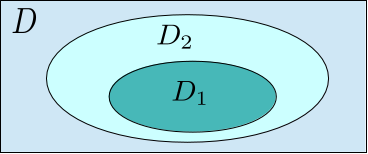
\includegraphics[width=0.75\linewidth]{./pic/solution_sets2}
		%\\ Здесь $D = 2^{\setN}$,
		
		$\displaystyle D_r = \arg \min_d \P^{(r)}(\Eps(d))$ {\footnotesize -- решения задачи выбора на основе оценок $r$-го эксперта, $D$ -- все решения.}
		
	     \end{center}
  
%	    \begin{gather*}
%		\mathsmaller{  \check{\p} \succ \p_1, \check{\p} \succ \p_2 }, \text{но: } \\ \forall\;\p' \neq \check{\p}, \p' \succ \p_1, \p' \succ \p_2: \p' \succ \check{\p}.
%	    \end{gather*}

	   \column{0.4\textwidth}
	     \begin{center}
	     	\hspace*{-2mm}    \tikz{ \node (otriv){   
      \begin{tikzpicture}  \begin{axis}[width = 32mm, height = 25mm,	xticklabels = {,,}, yticklabels = {,,}, ymin = -0.1, ymax = 1.1 ]
	\addplot[\mydarkgreen, ultra thick] table[x=xx, y=triv] {./pic/chapeter02-lattice2.dat};
       \end{axis}   \end{tikzpicture} };}
	     	    \vspace{2mm} 
		\\ \hspace*{-3mm} \tikz{ \node (osup){   
      \begin{tikzpicture}  \begin{axis}[width = 32mm, height = 25mm,	xticklabels = {,,}, yticklabels = {,,}, ymin = -0.1, ymax = 1.1 ]
	\addplot[\mydarkgreen, very thick] table[x=xx, y=sup] {./pic/chapeter02-lattice2.dat};
       \end{axis}   \end{tikzpicture}  };}
	    \end{center} 
	     \vspace{-3mm}
	     \begin{columns}
		  \column{0.5\linewidth}
		   \begin{center}
		      \tikz{ \node (oPP1){   
      \begin{tikzpicture}  \begin{axis}[width = 32mm, height = 25mm,	xticklabels = {,,}, yticklabels = {,,}, ymin = -0.1, ymax = 1.1 ]
	\addplot[\mydarkgreen, very thick] table[x=xx, y=pp1] {./pic/chapeter02-lattice2.dat};
       \end{axis}   \end{tikzpicture} };}
		     \vspace{2mm}
		  \\ \tikz{ \node (oP1){   
      \begin{tikzpicture}  \begin{axis}[width = 32mm, height = 25mm,	xticklabels = {,,}, yticklabels = {,,}, ymin = -0.1, ymax = 1.1 ]
	\addplot[\mydarkgreen, very thick] table[x=xx, y=p1] {./pic/chapeter02-lattice2.dat};
       \end{axis}   \end{tikzpicture} };}
		   \end{center} 
		  \column{0.5\linewidth}
		   \begin{center}
		     \tikz{ \node (oPP2){   
      \begin{tikzpicture}  \begin{axis}[width = 32mm, height = 25mm,	xticklabels = {,,}, yticklabels = {,,}, ymin = -0.1, ymax = 1.1 ]
	\addplot[\mydarkgreen, very thick] table[x=xx, y=pp2] {./pic/chapeter02-lattice2.dat};
       \end{axis}   \end{tikzpicture} };}
		      \vspace{2mm}
		  \\ \tikz{ \node (oP2){   
      \begin{tikzpicture}  \begin{axis}[width = 32mm, height = 25mm,	xticklabels = {,,}, yticklabels = {,,}, ymin = -0.1, ymax = 1.1 ]
	\addplot[\mydarkgreen, very thick] table[x=xx, y=p2] {./pic/chapeter02-lattice2.dat};
       \end{axis}   \end{tikzpicture} };}
		   \end{center} 
	      \end{columns}
	      \begin{center}
	          \vspace{-2ex}
		 {\small  Распределения образуют полурешётку. }
	     \end{center}
	\end{columns}
	
	\begin{tikzpicture}[overlay]
		\path[->] (otriv.south) edge  (osup.north);
		\path[->] (osup.south) edge  (oPP1.north);
		\path[->] (osup.south) edge  (oPP2.north);
		\path[->] (oPP1.south) edge  (oP1.north);
		\path[->] (oPP2.south) edge  (oP2.north);
	\end{tikzpicture}	
\end{frame} %===========================

\begin{frame}{Алгоритм коллективной экспертизы ($X$ конечно)}
 \begin{center}
      \vspace{-1ex}
	%{\small В конченом случае $\exists\ \underset{r \in R} \vee \p^{(r)}$  (супремум). Но его найти сложно. %Время $O\big(\abs{X}^{nm}\big)$ --- если <<в лоб>>. }%,  но его вычисление <<в лоб>> требует времени порядка $\abs{T} = \abs{X}^{nm}$. Найдём другую верхнюю грань.} 
	
	%В качестве коллективной экспертизы разумно использовать супремум. Но не можем его вычислить ($\abs{T} = \abs{X}^{nm}$). %Разработан только алгоритм вычисления супремума {\em одномерных} распределений. 
	%Что делать? Попробуем найти другую верхнюю грань, уточняемую оценками экспертов $\p^{(r)}$.
	%\textbf{Алгоритм} для конечного множества баллов $X$: 
	\vspace{-2mm}
	\begin{enumerate}
		\item ввести функции $v_r: X \times \setN \times \setM \rightarrow \zo$ 
		\\ $v_r(x, i, j) = \p_{ij}^{(r)}$, { \footnotesize $i = 1 \ldots n$, $j = 1 \ldots m$, $r = 1 \ldots R$, $x \in X$};
		\item рассчитать распределение $v = \underset{r \in R} \vee  v_r$ (супремум функций $v_r$); 
		\item выполнить обратное преобразование $\check{\p}_{ij}(x) = v(x, i,j)$ и полученные $\check{\p}_{ij}$  считать коллективным мнением экспертов, {\footnotesize $i = 1 \ldots n$, $j = 1 \ldots m$}.
	\end{enumerate}
	\vspace{-2mm}
	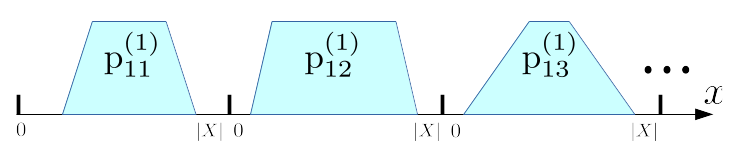
\includegraphics[width=0.85\linewidth]{./pic/glueon}
	\vspace{-1mm}
	 
	 Пусть $\p^{(r)}$ -- совместное распределение, полученное из оценок $\p_{ij}^{(r)}$, -- и совместное распределение $\check{\p}$ соотносятся как $\check{\p} \succ \p^{(r)}$  $\forall r = 1 \ldots R$. 
	 
	\textbf{Теорема:}  $\check{\p}$ есть верхняя грань множества $\{\p^{(r)} \mid r=\dotR\}$.
 \end{center}
\end{frame} %===========================


% == eof == eof ===